% Autor: Matthias Birnthaler

\section{Responsive Webdesign}

Für die Webseite wurde ein responsives Webdesign implementiert, so dass sie auf verschiedenen Geräten mit unterschiedlichen Aufklösungen dargestellt werden kann

\subsection{Auflösungen kleiner als 800 Pixel}
Der Kontent erstreckt sich nun über die ganze Seite. Die rechte und linke Spalte befinden sich nun unterhalb des Kontents und nehmen jeweils in etwa die Hälfte der Bildschirmauflösung ein.

\begin{figure}[!htbp]
\centering
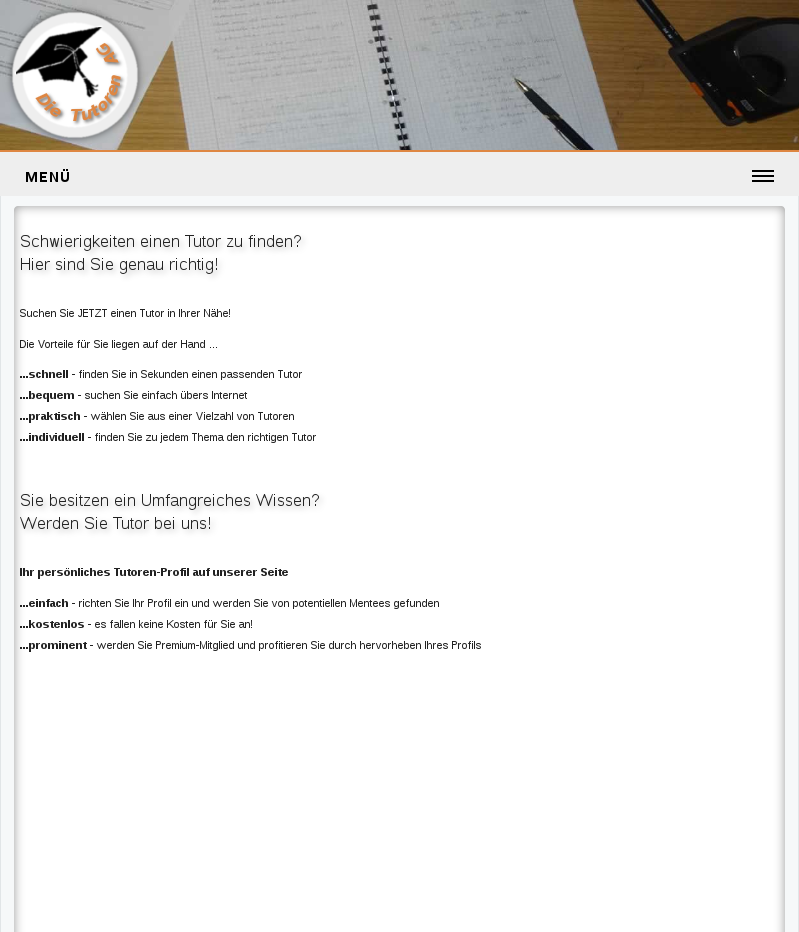
\includegraphics[scale=.55]{../Screenshots/responsive8001}
\caption{obere Webseitenhälfte}
\label{fig:responsive8001}
\end{figure}

\begin{figure}[!htbp]
\centering
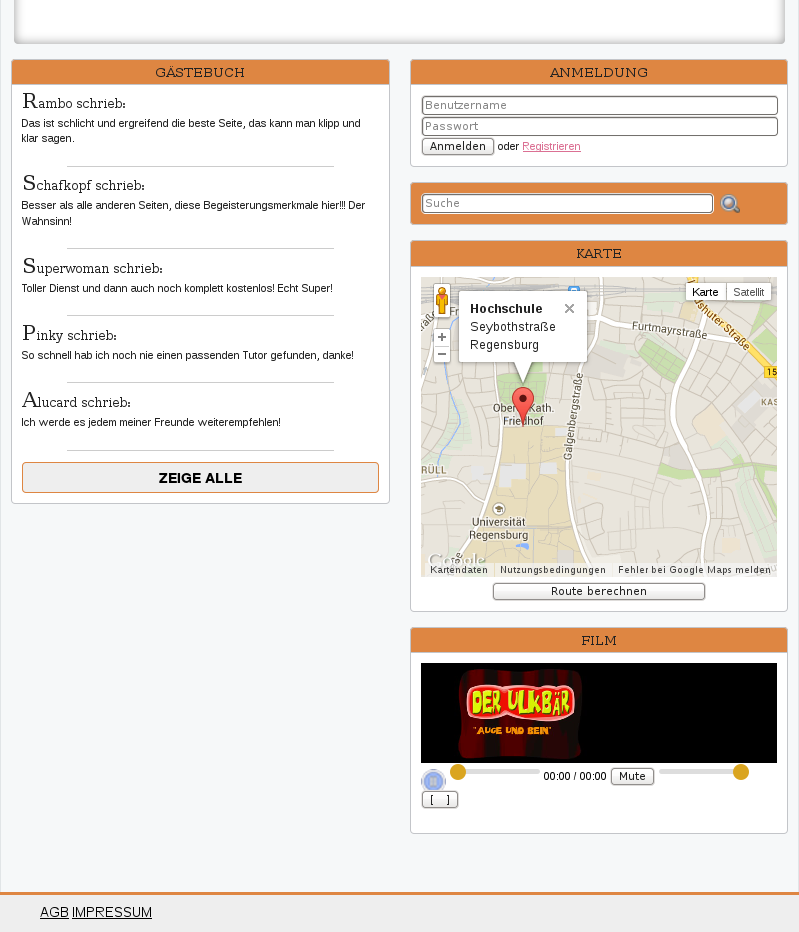
\includegraphics[scale=.55]{../Screenshots/responsive8002}
\caption{untere Webseitenhälfte}
\label{fig:responsive8002}
\end{figure}


\newpage

\subsection{Auflösungen kleiner als 400 Pixel}

Alle drei Spalten nehmen jeweils in etwa ganze Bildschirmauflösung ein und sind untereinander angeordnet. Der Kontent befindet sich ganz oben,  gefolgt vom rechten Balken un am Ende der linke Balken. Diese Anordnung wurde gewählt um die wichtigsten Inhalte am weitesten oben anzuordnen um einen schnellen Zugriff zu gewährleisten. Siehe Grafiken \ref{fig:responsive4001} und \ref{fig:responsive4002} auf den nächsten Seiten.


\begin{figure}[!htbp]
 \centering
 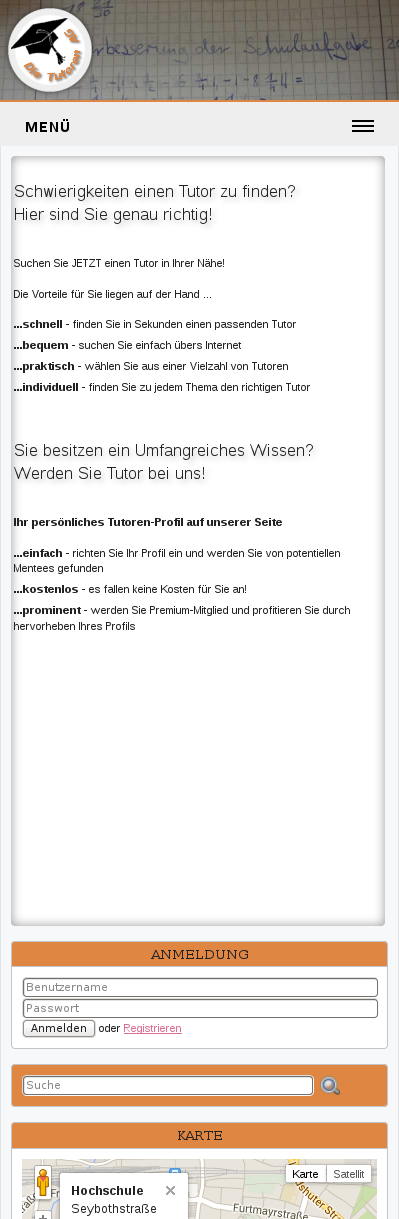
\includegraphics[scale=.55]{../Screenshots/responsive4001}
 \caption{obere Webseitenhälfte}
 \label{fig:responsive4001}
\end{figure}

\begin{figure}[!htbp]
 \centering
 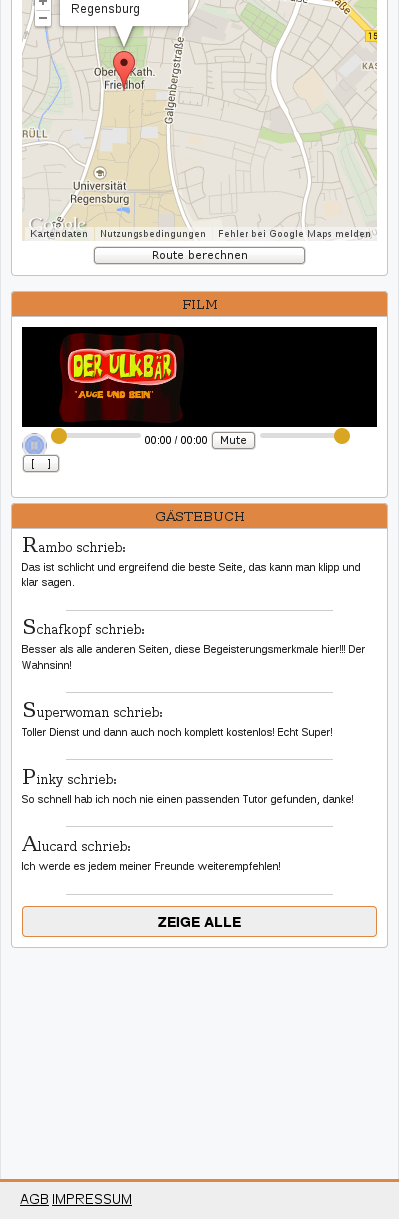
\includegraphics[scale=.55]{../Screenshots/responsive4002}
 \caption{untere Webseitenhälfte}
 \label{fig:responsive4002}
\end{figure}
